\documentclass[a4paper]{article}

%% Language and font encodings
\usepackage[english]{babel}
\usepackage[utf8x]{inputenc}
\usepackage[T1]{fontenc}

%% Sets page size and margins
\usepackage[a4paper,top=3cm,bottom=2cm,left=3cm,right=3cm,marginparwidth=1.75cm]{geometry}

%% Useful packages
\usepackage{amsmath}
\usepackage{graphicx}
\usepackage[colorinlistoftodos]{todonotes}
\usepackage[colorlinks=true, allcolors=blue]{hyperref}

\title{Analysis of Wait-Free Queues With Multiple Enqueuers and Dequeuers}
\author{Xiaohui Wang}

\begin{document}
\maketitle

\section{Introduction}

This paper analyzes the performance and implementation of a wait-free queue proposed by Alex Kogan and Erez Petrank \cite{1}. The lock-free data structures have been studied extensively. Lock freedom ensures that at least one thread will succeed to finish its operation among all threads. But the problem of lock freedom is that it might happens that one of the thread starves while trying to operate on the queue. On the other hand, wait freedom guarantees that a thread completes its operation withing bounded number of steps, as opposed to starvation. 

I implemented Kogan and Petrank's proposed wait-free queue in Go programming language. The repository can be found in \href{Wait-free queue}{github.com/wang502/wfqueue} . To better analyze the performance of the implementation, I also did several benchmarking on this wait free queue's operations (enqueue, dequeue). In the rest of the paper, I will give a detailed analysis on this wait free queue based on the benchmark data.
\section{Algorithm}

Kogan and Petrank's design uses a helping mechanism to ensure that each operation on the wait-free queue is completed in bounded number of steps. The way they achieve wait-freedom is by giving each thread (or operation) a age-based priority (a phase number) and making sure the threads with bigger phase numbers will help threads with smaller phases to complete. 

The wait-free queue has several important attributes: \textbf{head node}, \textbf{tail node} and a \textbf{state array}. A state array is an array of \textbf{OpDesc} objects which store the information of each thread's operation on the queue. The state array is initialized to be of length equal to the total number of threads. When doing enqueue/dequeue operation on the queue, by using the thread id as index, we can access and modify the corresponding State object in the state array. When each thread \textit{ti} starts an operation (enqueue/dequeue) on the queue, \textit{ti} chooses a phase number that is higher than all the phase numbers that the previous threads have chosen. Then the phase number along with some additional information are recorded in a Operation object, and the Operation object is stored in the state array at index i. 

Then thread \textit{ti} iterates over the \textbf{state} array. When iterating over the state array, it looks for OpDesc entries that have phase numbers smaller or equal to its phase number. The OpDesc entry that satisfies such criteria is operation left by other thread that is yet finished. So once \textit{ti} finds such an entry, it learns details about that thread operation by using that OpDesc entry, then it will try to help that thread execute its either enqueue of dequeue operation on the queue. 

\begin{figure}
\centering
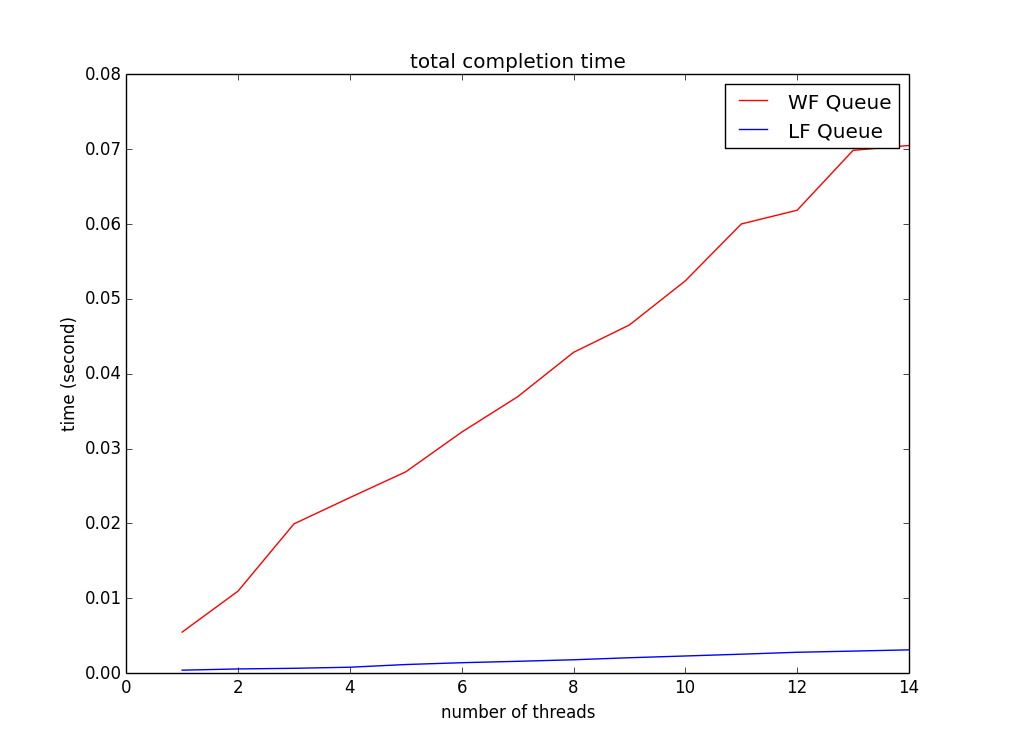
\includegraphics[width=0.66\textwidth]{benchmark1.png}
\caption{\label{fig:benchmark1}Benchmark result of all concurrent enqueue benchmark}
\end{figure}

\section{Benchmark}

In order to better evaluate the performance of this wait free queue, like what Kogan and Petrank stated in their paper, I also used compare the performance between wait-free queue and the lock-free queue proposed by Michael and Scott \cite{2}. The lock-free queue is also implemented in Go, same as the wait-free queue.
When evaluating the performance of wait-free queue, I use several benchmarks:
\begin{enumerate}
\item All concurrent enqueue: at the beginning, the queue is initialized as empty, then each thread iteratively enqueue items into the queue.
\item enqueue-dequeue pair: the queue is initialized as empty, each thread will first perform an enqueue operation followed by a dequeue operation
\end{enumerate}

For each benchmark, above, I measured the total completion time as the number of threads changes. For the first benchmark, each iteratively enqueues 1000 elements into the queue; and for the enqueue-dequeue pair benchmark, each thread performs enqueue-dequeue pair for totally 1000 times. I varied the number of threads between 1 and 14. 

\begin{figure}
\centering
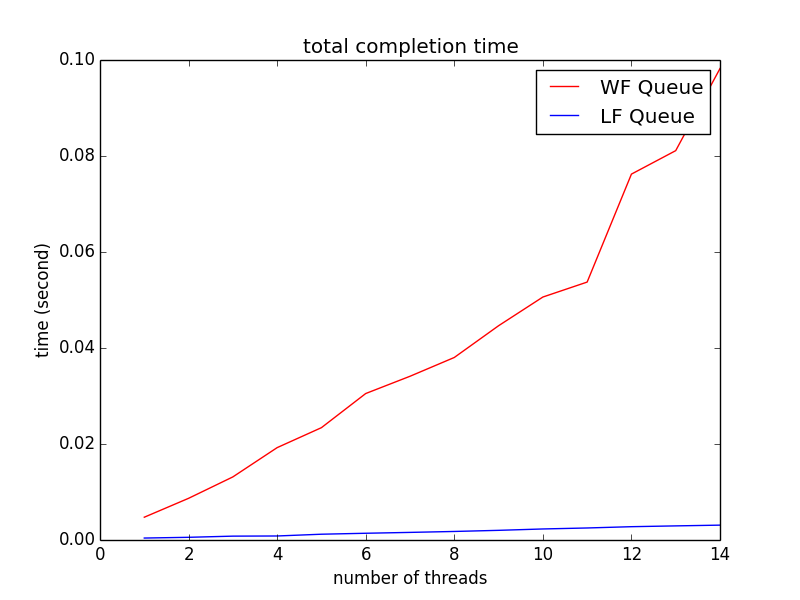
\includegraphics[width=0.66\textwidth]{benchmark2.png}
\caption{\label{fig:benchmark2}Benchmark result of enqueue-dequeue pairs benchmark}
\end{figure}

Figure 1 shows the result for the first benchmark. Overall, the performance for lock-free queue is better than the wait-free queue. And as the number of threads increases, the completion times increases much faster for wait-free queue than for lock-free queue. As we can see a steeper slope for wait-free queue. 

Figure 2 shows the result for the second benchmark, where each thread iteratively performs enqueue operation followed by a dequeue operation. Same as the result of first benchmark, it takes less time for lock-free queue to complete all operations than wait-free queue. And the completion time of wait-free queue increases more as the number of threads increases. And notice that, for wait-free queue, once the number of threads surpass 12, the completion increases even much more than before. 

\section{Analysis}
Through analyzing the implementation of Wait-free queue that Kogan and Petrank proposed, we can find that this wait-freedom is achieved with the prices of some overhead that possibly slow the program down.

\begin{figure}
\centering
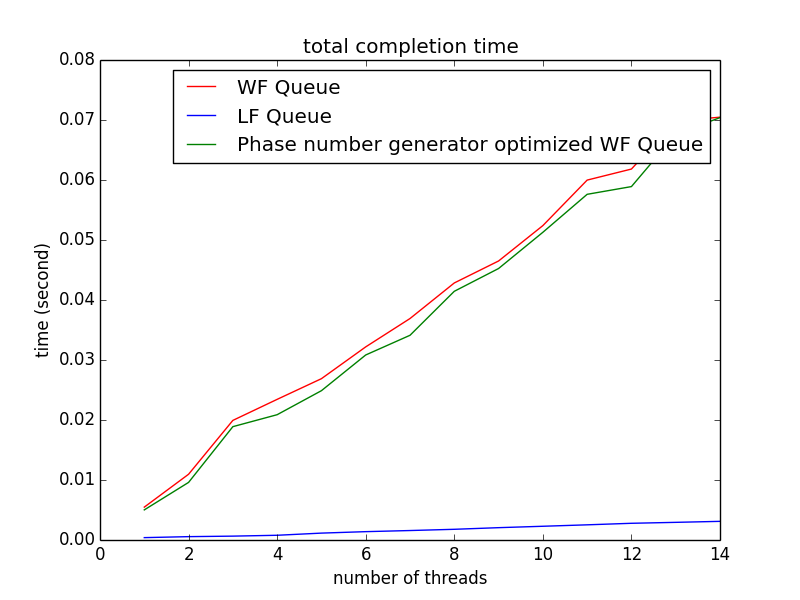
\includegraphics[width=0.66\textwidth]{benchmark3.png}
\caption{\label{fig:benchmark3}Benchmark result of all concurrent enqueue benchmark, with Wait-free queue's phase number generator optimized}
\end{figure}

One of the notable overhead occurs in the phase number generation when each thread starts its operation on the thread. In the implementation they proposed, in order for a thread to get its phase number, it needs to loop through the \textbf{state array}, and among those \textbf{OpDesc} entries, find the maximum phase number that already been taken by the previous operations, and increment that maximum phase number by 1. As the number of threads increases, the length of state array increases, and the overhead will be even more obvious. This leads to first optimization:
\begin{itemize}
\item Keeping an atomic integer in the queue structure, as also proposed by Kogan and Petrank
\end{itemize}
By having an atomic integer \textit{curPhase} in the queue structure, every time a thread wants to get its phase number, it simply needs to do an atomic CAS operation that atomically increments the current phase number by one and then obtain the new phase number. In this way, it will be more efficient than the previous way. As is shown in Figure 3, which shows the first benchmark, with the wait-free queue that has faster phase number generation. The green line shows the completion time of optimized wait-free queue with better phase number calculation. It is obvious that the optimized one behaves better that the original wait-free queue, although the lock-free queue still performs the best. 

\begin{figure}
\centering
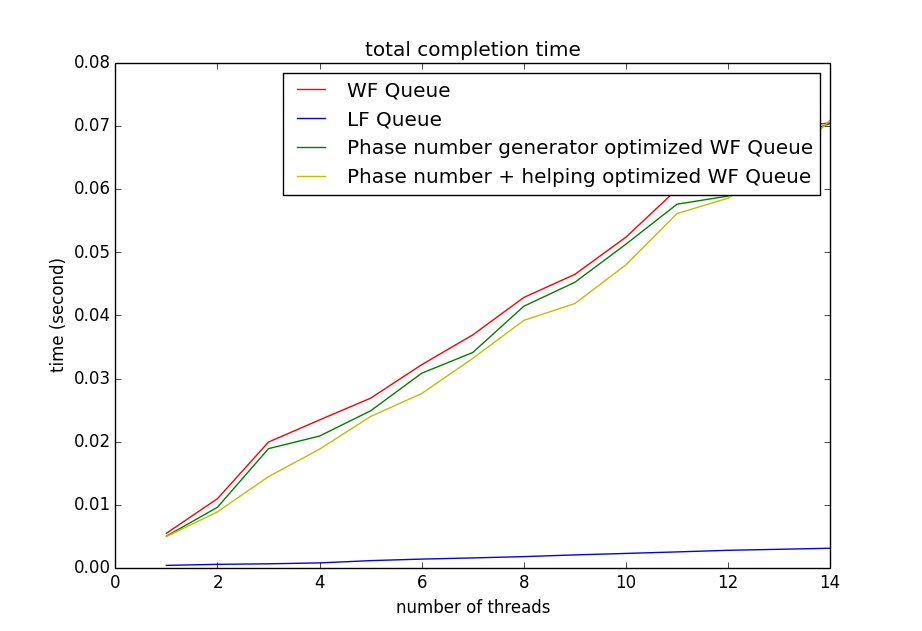
\includegraphics[width=0.66\textwidth]{benchmark4.png}
\caption{\label{fig:benchmark4}Benchmark result of all concurrent enqueue benchmark, with Wait-free queue's phase number generator and helping mechanism optimized}
\end{figure}

Another notable overhead happens when many threads are trying to help the same thread to complete its operation. In this scenario when several threads are helping the same thread, the synchronization of those threads waste much computation time. Since if one thread \textit{ti} is able to help thread \textit{tj}, there is no need of another thread to help \textit{tj} any more. Thus, to avoid this repeating computation, we need a slight modification of the helping mechanism. This leads to second optimization:
\begin{itemize}
\item Having one thread help at most one thread, instead of more, as original implemented
\end{itemize}

As is defined in \textbf{wfqueue.go}, the function help() from line 172 to 189: a thread that calls help will iterate over the state array, look for pending thread operations that have smaller phase numbers, and help those threads finish the operations.The original implementation comes without the return statement on line 186. The optimization is adding the return statement on line 186. In this way, thread \textit{ti} calling the help function, only help at most one thread and then returns. Figure 4 shows the performance with this optimization. The yellow line shows the changes in completion time of wait-free queue with phase number calculation and helping mechanism optimized as thread number increases. As we can see, the performance gets even better with both optimizations. Since now one thread only help at most thread, the scenario where various threads fighting to help the same thread will occur less, thus the performance becomes better.

\section{Conclusion}
Kogan and Petrank's wait-free queue guarantees wait-freedom by using the helping mechanism, which lets new threads help older threads. When several threads are trying to help the same thread to complete its operation, the synchronization between those threads slows the operation down. But the good thing about this wait-freedom is that every thread is guaranteed to finish in a bounded number of steps, as Kogan and Petrank puts it: equal to the length of \textbf{state} array. So this proposition of new wait-free queue does not bring much practical benefits in terms of usage. Because the performance will become a huge bottleneck. When I try to run the wait-free queue with more than 20 threads, the program takes a very long time to finish. So sacrificing the performance in exchange of wait-freedom seems not worthwhile, but it is definitely worth knowing the concept of helping mechanism among those threads.

\bibliographystyle{alpha}
\bibliography{sample}

\end{document}